\documentclass[compress]{beamer}

\mode<presentation>
\usetheme{Singapore}
\usecolortheme{rose}

% \usepackage{amsmath,amsfonts,amssymb}
% \usepackage{colortbl}
% \usepackage{hyperref}
\usepackage{tikz}
\usetikzlibrary{calc}
\usetikzlibrary{positioning}
\usetikzlibrary{calc,intersections,through,backgrounds}

%%% Template Setting

%% Font
\usefonttheme[onlylarge]{structuresmallcapsserif}
\usefonttheme[onlysmall]{structurebold}
\setbeamerfont{title}{shape=\itshape,family=\rmfamily}
\setbeamertemplate{frametitle}[default][center]


\title{Molding CNNs for text: non-linear, non-consecutive convolutions}
\author{Tao Lei, Regina Barzilay, and Tommi Jaakkola}
\institute{Presented by Shih-Ming Wang \\ NLPLab, Institute of Information Science, Academia Sinica}
\date{07-5-2016}
\subject{Computer Science}

\graphicspath{{img/}}

\begin{document}
\beamertemplatenavigationsymbolsempty

\begin{frame}
 \maketitle
\end{frame}

\begin{frame}
 \frametitle{Outline}
 \tableofcontents
\end{frame}

\section{Introduction}
    \begin{frame}{\secname}
        \begin{block}{Motivation}
            \begin{itemize}
                \item Deep learning \& Convolution neural network (CNN) have led to success in many NLP problems
                \item Convolution operation is a \textbf{linear} mapping over \textbf{n-gram} vectors
                \item Target: \textbf{non-linear} operation over \textbf{non-consecutive} n-grams (e.g., ``\underline{not} that \underline{good}'')
            \end{itemize}
            
        \end{block}
    \end{frame}

\section{Background}
    \begin{frame}{\secname}
        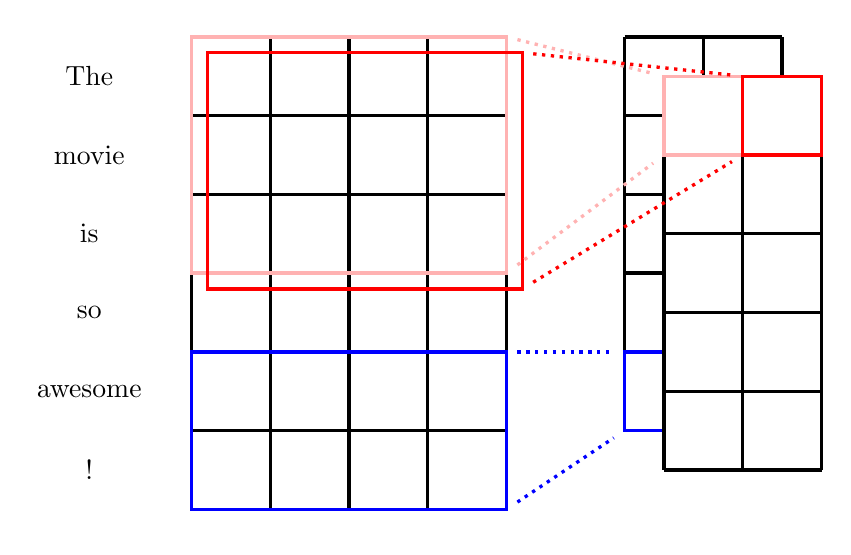
\begin{tikzpicture}
            [border/.style={very thick},
            link/.style={very thick, dotted},
            ]
            \colorlet{f1color}{red!30!white}
            \colorlet{f2color}{red}
            \colorlet{f3color}{blue}
            \begin{scope}[shift={(0,0)}]
                \begin{scope}[shift={(-1.3,.5)}]
                    \node at (0,5) {The};
                    \node at (0,4) {movie};
                    \node at (0,3) {is};
                    \node at (0,2) {so};
                    \node at (0,1) {awesome};
                    \node at (0,0) {!};
                \end{scope}

                \draw[border, step=1cm] (0,0) grid +(4, 6);
                \draw[border, f1color] (0,3) rectangle +(4, 3) node(A1){} +(4,0) node(A2){};
                \draw[border, f2color] (.2,-.2) ++(0,3) rectangle +(4, 3) node (B1){} +(4,0) node(B2){};
                \draw[border, f3color] (0,0) rectangle +(4,2) node(C1){} +(4,0) node(C2){}; 

                \begin{scope}[shift={(5.5, 1)}]
                    \draw[border, step=1cm] (0,0) grid +(2,5);
                    \draw[border, f3color] (0,0) node(C4){} rectangle +(1,1) +(0,1)node(C3){};
                    \fill[white] (0.5,-0.1) rectangle (2.1,4.5);

                    \begin{scope}[shift={(0.5,-.5)}]
                        \draw[border, step=1cm] (0,0) grid +(2,5);
                        \draw[border, f1color] (0,4) node(A4){} rectangle +(1,1) +(0,1)node(A3){};
                        \draw[border, f2color] (1,4) node(B4){} rectangle +(1,1)  +(0,1)node(B3){};
                    \end{scope}
                \end{scope}
                \draw[link, f1color] (A1) -- (A3);
                \draw[link, f1color] (A2) -- (A4);
                \draw[link, f2color] (B1) -- (B3);
                \draw[link, f2color] (B2) -- (B4);
                \draw[link, f3color] (C1) -- (C3);
                \draw[link, f3color] (C2) -- (C4);
            \end{scope}
        \end{tikzpicture}
    \end{frame}

\section{Model Description}
        \begin{frame}[allowframebreaks]{\secname}
            \begin{block}{Tensor-based Feature Mapping}
                \begin{itemize}
                    \item Use outer product operation instead of linear combination
                    \item Consider 2-gram $(x_1, x_2)$ (row vectors) as example:
                \end{itemize}
                \begin{table}[t]
                    \centering
                    \begin{tabular}{lrrr}
                                & Linear             & Outer Product        & 3D case                             \\ \hline
                    Raw         & $[x_1; x_2]$       & $x_1^T \cdot x_2$    & $x_1 \bigotimes x_2 \bigotimes x_3$ \\ \hline
                    Dim(raw)    & $2\times d$        & $d\times d$          & $d\times d \times d$                \\ \hline
                    Dim(Kernel) & $h\times2\times d$ & $h\times d \times d$ & $h\times d \times d \times d$       \\ \hline
                    Output      & $h\times 1$        & $h \times 1$         & $h \times 1$
                    \end{tabular}
                \end{table}
                ,where $(x_1 \bigotimes x_2 \bigotimes x_3)_{ijk} = x_{1i} \cdot x_{2j} \cdot x_{3k}$
            \end{block}
        \framebreak
            \begin{block}{Parameter Explosion}
                \begin{itemize}
                    \item Kernel $T$ has $h\times d^n$ parameters for n-gram
                    \item Solution: Decompose $T$ in to sum of $\bar{h}$ rank-1 tensors
                    \begin{table}[t]
                    \centering
                    \begin{tabular}{lll}
                            & 2D                                                              & 3D
                           \\ \hline
                    Dim(T)  & $h\times d \times d$                                            & $h\times d \times d \times d$                                                  \\ \hline
                    T'      & $\sum\limits_{i=1}^{\bar{h}} O_i \bigotimes P_i \bigotimes Q_i$ & $\sum\limits_{i=1}^{\bar{h}} O_i \bigotimes P_i \bigotimes Q_i \bigotimes R_i$ \\ \hline
                    \end{tabular}
                    \end{table}
                    ,where\\
                    $O \in \mathbb{R}^{\bar{h} \times h}$; $P, Q, R \in \mathbb{R}^{h\times d}$; \\
                    $O_i \in \mathbb{R}^h$; $P_i, Q_i, R_i \in \mathbb{R}^d$

                    For simplity, $\bar{h}=h$.
                \end{itemize}
            \end{block}
        % \framebreak
            % \begin{block}{Feature Map Calculation}
                % \begin{table}[t]
                % \centering
                % \begin{tabular}{lll}
                %         & 2D                                                              & 3D                                                                             \\ \hline
                % Feature & $x_1 \bigotimes x_2$                                            & $x_1 \bigotimes x_2 \bigotimes x_3$                                            \\ \hline
                % Kernel  & $\sum\limits_{i=1}^{\bar{h}} O_i \bigotimes P_i \bigotimes Q_i$ & $\sum\limits_{i=1}^{\bar{h}} O_i \bigotimes P_i \bigotimes Q_i \bigotimes R_i$ \\ \hline
                % Output  & $O \cdot (Px_1 \bigdot Qx_2)$                                   & $O \cdot (Px_1 \bigdot Qx_2 \bigdot Rx_3)$
                % \end{tabular}
                % \end{table}
                % ,where $\bigdot$ is element-wise product. \\
                % \begin{itemize}
                %     \item $Px_1$ is a linear transformation of $x_1$
                %     \item Higher-order terms (i.e. $x_1 \bitotimes x_2 \bigotimes x_3$) arise from the element-wise products.
                % \end{itemize}
            % \end{block}
            

        \end{frame}


\section{Experiments}
\begin{frame}{\secname}
\end{frame}

\section{Error Analysis}
\begin{frame}{\secname}
\end{frame}



\end{document}
